\chapter{Présentation du stage}

Mon stage a commencé le lundi 10 juin 2024. Après avoir récupéré un ordinateur et un PIN-pad générateur d'OTP (One-Time-Password), Carlos, mon maître de stage a pu me montrer comment comprendre la librairie que j'allais développer : Antares. Une ressouce sur l'intranet ? permet d'apprendre à l'utiliser. Pour vous illustrer la base d'une solution CFD que nous pourrions vouloir traiter avec Antares, voici un schéma :

\begin{figure}[h!]
    \centering
    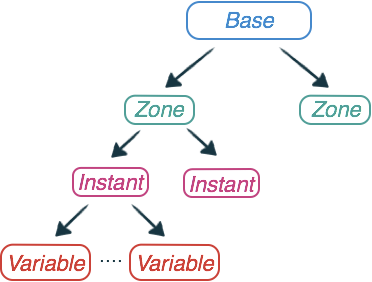
\includegraphics[width=0.5\textwidth]{images/data_structure_1.png}
    \caption{Structure des données} %\footnote{Source:https://cerfacs.fr/antares/src/tutorial/base.html}}
    %\label{fig:https://cerfacs.fr/antares/src/tutorial/base.html}
\end{figure}


Ensuite, j'ai été chargé de résoudre un petit bug sur Antares, ce qui m'a permis de prendre la main sur Nitrox, le gitlab hébergé sur le serveur du CERFACS où se situe Antares et d'autres codes du CERFACS.

\section{Mission 1 : Les différentes méthodes d'interpolation}
Ma première mission a été de recensser les méthodes d'interpolation qui seraient implémentables dans Antares, à savoir, qui permettent de l'interpolation 3D, sur des maillages dits non structuré, c'est à dire pas de simples maillages, rectangulaires en 2D et hexaédrique en 3D, représentés par des matrices, mais des maillages créés avec différentes formes géométriques.
Le temps de calcul, appelé 'coût' est aussi un paramètre à prendre en compte.
Finalement, les caractéristiques des équations à interpoler est probalement le paramètre le plus important à prendre en compte mais aussi assurément le plus difficile. Effectivement différentes équations très difficiles à caractériser tel que l'équation de Naviers-Stokes sont utilisées et mon niveau en maths est trop limité pour pouvoir me plonger en profondeur dans ce problème. C'est pour cela que je n'ai pas de résultat mathématique à présenter dans cette partie. Mais heuresement que ces méthodes ont déjà été implémentés et testés pour d'autres codes de simulation numérique, ce qui donne une bonne idée des résultats que nous pouvons espérer.

%\addcontentsline{toc}{section}{L'interpolation et l'aéroacoustique}

\subsection{L'interpolation par voisin le plus proche}
Cette première méthode est très simple : nous prenons comme valeur \( v \) d'interpolation au point \( p \) la valeur \( v \) du point le plus proche de \( p \).
Nous comprenons assez vite que cette méthode est discontinue et même pas linéaire...
Nous pouvons aussi imaginer que 2 points à droit et à gauche d'une ligne horizontale de 3 points (les plus proches), prendrons la même valeur pour \( N \) = 3, Schématiser. 

D'autres méthodes dérivés ou similaiers existent pour évaluer nos poids. La plus intéressante serait celle dite de Franke-Littke. Elle consiste à utiliser une distance maximal autour du points au-delàs les autres points ne sont pas pris en compte. Autrement dit, en utilisant un cercle (dans le cas 2D) d'un certain rayon pour déterminer quels points nous sont utile pour l'interpolation. Dans ce cas le nombre de points est variable.
J'ai considéré subjectivement que cette méthode n'étais pas intéressante car, confronté à un maillage ayant une différence de rafinement intrinsèque importante, dans certains cas aucuns points ne seraient pris, et dans d'autes, une grande somme serait calculée.


\begin{comment}
Certaines conditions de cette méthode doivent être respectés, comme Pour N tends vers l’inf, p doit être inférieur ou égale à la dimension, par ex 3 pour ne pas diverger. Mais N n’est pas grand dans notre cas.
Voir d'autres choses page 7 de mon ppt.
\end{comment}


\subsection{L'interpolation IDW}
\[
\hat{f}(x) = \frac{\sum_{i=1}^{N} \frac{f(x_i)}{d(x, x_i)^p}}{\sum_{i=1}^{N} \frac{1}{d(x, x_i)^p}}
\]

où :

- \(\hat{f}(x)\) est la valeur interpolée à la position \(x\),

- \(f(x_i)\) est la valeur connue aux points de données \(x_i\),

- \(d(x, x_i)\) est la distance entre \(x\) et \(x_i\),

- \(p\) est le paramètre de puissance,

- \(N\) est le nombre total de points de données.



Probablement l'iterpolation la plus simple après la méthode du voisin le plus proche (toujours dans notre cas d'application), cette méthode est la seule qui étais implémenté dans Antares.

Nous pouvons modifier 2 paramètres : \(p\) et \(N\).
Par défault, dans le code, \(p\) = 1 et \(N\) est égale aux nombres de sommets de la première forme de cellule de la liste de formes de cellules de la base target (je n'ai pas compris pourquoi pas de la base source) /! Tests à faire ici /!
Ces informations ne sont pas confidentielles Carlos ?

Nous remarquons que pour \( n = 1 \), nous retrouvons la méthode du voisin le plus proche, pour tout \( p \).

Une de mes mission étais de chercher s'il y avait des paramètres plus optimisés que \(N\) et \(p\) pour cette méthode. Je n'ai pas trouvé le réponse dans les différents articles et thèses que j'ai lu. C'est pour celà que je présenterais plus tard comment j'ai trouvé des paramètre optimaux en faisant des tests.


\subsection{L'interpolation polynomiale}
\subsection{L'interpolation par Splines}
\subsection{Méthodes géostatiques}
\subsection{Méthode par moindres carré}
\subsection{MISCOG}

\subsection{L'interpolation (tri)linéaire   A METTRE EN DERNIER POUR AVOIR UNE BELLE TRANSISTION ?}
Aussi appelée interpolation Barycentrique, l'inerpolation linéaire, est la plus simple (après les plus proches voisins et IDW), et la plus utilisée par Aibus, Safran et d'autres industriels (dans via d'autres codes qu'Antares).
C'est pour cela qu'ils ont demandé au CERFACS de l'implémenter des antares, car ils l'utilisent actuellement via d'autres moyen.
En 1D, l'interpolation linéaire est simple : c'est la moyenne pondérée linéairement par la distance, des valeurs des points.
Supposons que nous voulons interpoler une valeur d'un point \( p \) entre deux points \( a \) et \( b \) dans un espace 1D
et que nous représentons leurs valeurs dans une deuxième dimension \( y \).
Nous aurons alors pour formule :

\[
y_p = \frac{x_b - x_p}{x_b - x_a} \cdot y_a + \frac{x_p - x_a}{x_b - x_a} \cdot y_b
\]

%\vspace*{0.1\baselineskip}\linebreak
où \( y_p \) représente la valeur interpolée à la position \( x_p \), et \((x_a, y_a)\) et \((x_b, y_b)\) sont les points de référence. J'ai écris cette formule afin qu'elle soit symétrique par rapport aux points \( a \) et \( b \), pour qu'il jouent la même rôle. Ainsi elle s'entendra plus intuitivement dans des dimensions supérieurs.
%\vspace*{0.1\baselineskip}\linebreak

        \( \frac{x_b - x_p}{x_b - x_a} \) est le poids pour \( y_a \) basé sur la distance relative de \( x_p \) à \( x_b \).

        \( \frac{x_p - x_a}{x_b - x_a} \) est le poids pour \( y_b \) basé sur la distance relative de \( x_p \) à \( x_a \).%\\

Ces deux termes sont pondérés de manière à ce que leur somme soit toujours égale à 1, ce qui garantit que l'interpolation est correcte et symétrique par rapport à \( a \) et \( b \).

En 2D, nous devons nous baser sur des surfaces, extraites de formes pour pouvoir effectuer cette pondération. En CFD (Computation Fluid Dynamics en anglais), ces formes sont appelés cellues et leurs sommets noeuds. Dans notre cas, nous considérons que les variables du maillages sont contenus au niveau des noeuds. Aussi, Antares ne traites que des maillages ayant des valeurs uniquement au niveau des noeuds des cellules (pas entre).
Il existe 2 principales types de cellules (formes) en 2D : les triangles et les quadrilatères (non croisés).
% Pour le triangle, la méthode pour trouver la valeur au point à interpoler \( p \) est celle dite du barycentre (barycentrique). // Pour les autres formes aussi.
L'interpolation barycentrique pour un triangle est bien documentée. Visuellement, il faut faire la somme des valeurs au points pondéré par la surface opposé et pondéré le tout par la surface du triangle. % Expliquer mathématiquement ? Ou plus tard dans le code ? 



% (quadrilatère non croisé, concave et convexes)
% En CFD il y a toujours des formes, même si c'est structuré, on peut unstructure.

\subsection{Resumé des similitudes et différences des différentes méthodes}



\section{L'implémentation de la méthode trilinéaire}
%\subsection{La prise en main de la libraire Antares}
\subsection{L'algorithme}
\subsection{Les difficultés}
\subsection{Le résultat}



\section{Les tests sur des cas d'aéroacoustique}
% \section{Les différentes méthodes d'interpolation}
Carlos a développé l'outils permettant de déterminer le résultat acoustique, à grande distance, à partir d'un surface, en utilisant les équations de Ffowcs Williams – Hawkings. Le résultat acoustique sont les petites variations de pression, impliquant du son (à différentes fréquences et amplitudes). En pratique, pour les utilisateurs d'Antares, cette surface est définie dans un maillage 'solution' où nous avons le résutlat de la pression en différents points et différents instants.
% Paramètres d'IDW
\subsection{Tests sur les paramètrs de la méthode IDW}




... (\url{https://cerfacs.fr/antares/}) : 


\begin{itemize}
    \item TreeMesh 
    %Ici, le maillage DGMultiMesh dépend directement du solver DGMulti en fonction du type de géométrie utilisée, il faut donc le passer en argument.
\end{itemize}


\subsection{Discrétisation spatiale et résolution du problème}